\section{Tidal circularization}
%
\label{sec:synchronization_circularization_alignment}

The effect of tides scales as the difference in the gravitational acceleration
due to the companion at the near and far tidal bulges multiplied by the mass in
each bulge. Both of these factors themselves are a strong function of the ratio
of the size of the object to the size of the orbit. As a result, the tidal
coupling between a planet and its host star decreases very rapidly as the
distance between the planet and the star increases. This is why tides are only
important for planets which get very close to their parent stars at least for
some part of their orbit.

As described in the previous section, planetary tides exchange angular
momentum between the orbit and spin of the planet, stellar tides exchange
angular momentum between the orbit and spin of the star, and both tides extract
energy out of the system, leading to orbital circularization.

The quantity that is most readily affected by tides is the spin of the planet.
This is due to two reasons. First, the angular momentum of the planet is many
orders of magnitude smaller than both the orbital and stellar angular momenta,
so it most easily affect. Second, the self-gravity of the planet is much smaller
than that of the star, and the tidal force on the planet is much larger than
that on the star. Since the size of the tidal bulges is determined by the
competition between self-gravity and tidal force, the planetary tides are much
stronger. As a consequence, the expectation is that pseudo-synchronizing the
planet's spin with the orbit should be the tidal signature affecting the largest
number of exoplanet systems. Unfortunately, at present, there is no way to
observationally determine the spin of an exoplanet, so we cannot test this
prediction.

\begin{figure}[t]
%
    \centering
%
    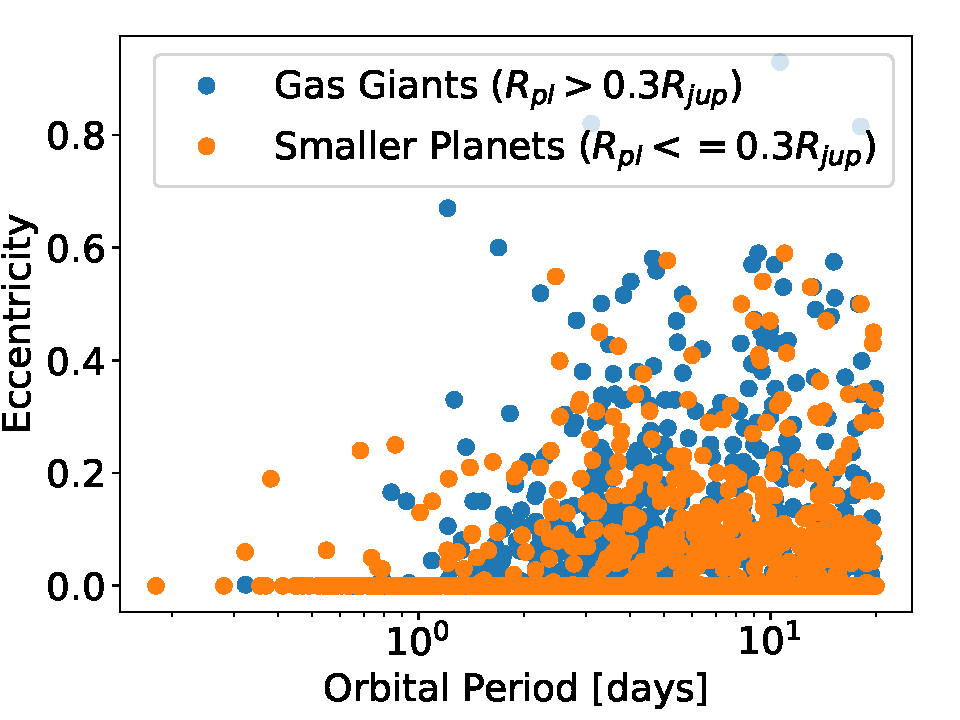
\includegraphics[width=0.5\textwidth]{period_eccentricity.pdf}
%
    \caption{
%
        The period vs eccentricity of the currently confirm extrasolar planets
        from the NASA exoplanet archive. The color indicates the radius of the
        planet.
%
    }
%
    \label{fig:period-eccentricity}
%
\end{figure}

The second most strongly tidally affected property of exoplanet systems is the
eccentricity of their orbits. For most systems the orbital angular momentum is
smaller than the stellar spin angular momentum and it is feeling the combined
effect of both stellar and planetary tides, with the latter being significantly
more important as long as the eccentricity is not negligible. The observational
evidence of tides on the orbital eccentricity is that the shorted period
systems, which experience the strongest tides, get circularized very quickly, so
they are all observed in circular orbits, with gradually more and more
eccentricity surviving at longer and longer orbital periods (see
Fig.~\ref{fig:period-eccentricity}).

\section{Tidal inspiral}

Another effect that is expected to occur in very short period exoplanet systems
is tidal inspiral. This is only relevant for exoplanet systems whose orbital
period is short enough for the tides on the planet to have circularized the
orbit and synchronized the spin of the planet with it. As a result, the
planetary tides are now static on the surface of the planet and no longer
experience friction. This leaves only stellar tides to drive further evolution.
Stars generally have spin periods exceeding the orbital period. As discussed
above, this situation leads to tidal bulges that lag behind the planet as it
move around in its orbit, leading to removal of angular momentum from the orbit
and adding it to the spin of the star. Since stars have hundreds to thousands of
times more mass than even the most massive planets, their moment of inertia is
in almost all cases large enough to prevent the star from synchronizing to the
orbital period of the planet. As a result, stellar tides gradually shrink the
orbit of the planet, driving it closer and closer to the star.

If the planet starts out relatively far away from the star, this inspiral could
take longer than the lifetime of the star, but for the shortest period systems,
this will eventually push the planet close enough to its parent star for one of
two things to happen. First, tides get stronger as the planet-star separation
decreases, until the tidal force attempting to stretch the planet overwhelms the
self-gravity of the planet. This will cause the planet to be tidally ripped
apart. The distance between the planet and the star at which this occurs is
known as the Roche limit, and it depends on the size and mass of the planet. The
more massive the planet is, the stronger its self gravity, pushing the Roche
limit closer to the star.  Similarly, the larger the planet, the weaker its self
gravity, and hence the Roche limit is pushed further away. In the case of gas
giant planets, the Roche limit is comparable to the size of the star. For some
planets, it lies inside the star, in which case the planet will be engulfed by
the star still relatively intact. In either case, the tidal inspiral will cause
the destruction of the planet.

Two separate lines of evidence point to this process occurring for gas giant
exoplanets, while perhaps not for smaller, rocky planets. First,
\citep{Jackson_et_al_09} pointed out that the smallest orbits in which younger
exoplanet systems are observed are smaller than the smallest orbits in which
older systems are observed. This is matches the predictions of the tidal
inspiral scenario, as the older systems have more time to be affected by tides
and hence systems beginning with larger separations will inspiral and be
destroyed. A different line of evidence for the tidal destruction of the
shortest orbital period exoplanets comes from their velocities within the
galaxy. \citep{Hamer_Schlaufman_19} compared the host stars of giant planets in
orbits with periods few days (a.k.a. hot Jupiters) to two control samples of
stars without planets, and stars with longer period planets. What they found is
that the velocities of hot Jupiter hosts show much smaller scatter around the
mean rotation of the galaxy less than either of the control samples, while the
distribution of velocities of the two control samples are statistically
indistinguishable. It is a well established property of our galaxy that the
smaller the scatter in the velocities of a sample of stars, the younger it is.
Hence, this observation is another indication of the relative youth of systems
containing short period giant planets, suggesting the older systems have lost
their planets to tidal inspiral.

\section{Tidal alignment}

The tidal torque due to the stellar tides on the orbit will also cause the orbit
to align with the equator of the star. This is one of the leading explanations
for the observed trend that giant planets orbiting Sun-like stars appear to
have orbits that are aligned with the stellar equator, while stars significantly
more massive, and hence hotter, than the sun, seem to host planets with all
kinds of orbital orientations \citep[c.f. chapter 5.2 of][]{Winn_Fabrycky_2015}.
The lack of alignment between hot stars and the orbits of their companion
planets has been hypothesized to be due to much weaker tidal friction that is
expected to occur in these stars. More specifically, the transition between
aligned and mis-aligned orbits appears to coincide with the transition between
stars that have surface convective zones and those that do not, and the
turbulent flow present in stellar convective zones has long been thought to be
one of the leading causes of tidal friction.

It must be emphasized, however, that the tidal interpretation of the observed
alignment pattern is far from universally accepted.  Alternative suggestions
include the possibility that most planets generally form aligned, with various
mechanisms causing misalignment in some systems.
